\section{Evaluation}
% 	Around 2 - 3 pages
%     - Reference implementation
%      * Base reference
%     - Testing, and how it was done
%     - Different stages of implementations
%     - Compare
% -----



An evaluation can me made using the data gotten using the test scripts described in the implementation section \ref{section-Implementation}. All measurements is measured by counting the cycles it takes to run the code.

\subsection{Testing}
Testing was done using the setup described in subsection \ref{sub-testing}. This enables testing of different seeds, Karatsuba operand lengths and multiple iterations of the algorithm.


\subsection{Reference implementation}
The reference implementation uses Montgomery ladder approach for point multiplication, schoolbook multiplication, and branch less fixed time approaches to the arithmetic in general. This makes it easier to measure the cycles as it they wont change depending on its input. The reference implementation takes $79.794$ megacycles to run.

\subsection{Karatsuba}
The testing method described in \ref{karatTesting} has been used to find the best operand length for the Karatsuba algorithm. The results of the test scripts has been plotted into a chart, and can be seen in figure \ref{karatsubafigure}. Based on those results the best operand length must be $32$, as this results in the least cycles. \\ 
\begin{figure}[H]
\begin{subfigure}{\textwidth}
    \centering
    \fbox{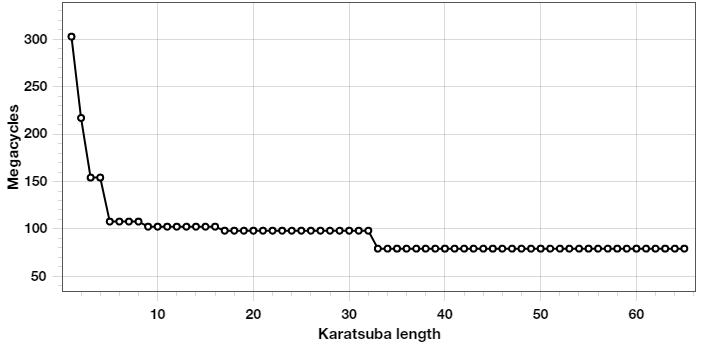
\includegraphics[width=0.8\textwidth]{report/images/karatsuba.png}}
    \caption{Karatsuba operand length - cycles}
\label{karatsubafigure}
\end{subfigure}
\end{figure}
Using this operand length results in a measurement of $79.118$ megacycles. To compare the Karatsuba cycles with the reference implementation both have been plotted into a chart in figure \ref{karatsubacomparison}. This chart shows the difference between the two implementation is not magnificent, as the difference is $0.676$ megacycles.\\

\begin{figure}[H]
\begin{subfigure}{\textwidth}
    \centering
    \fbox{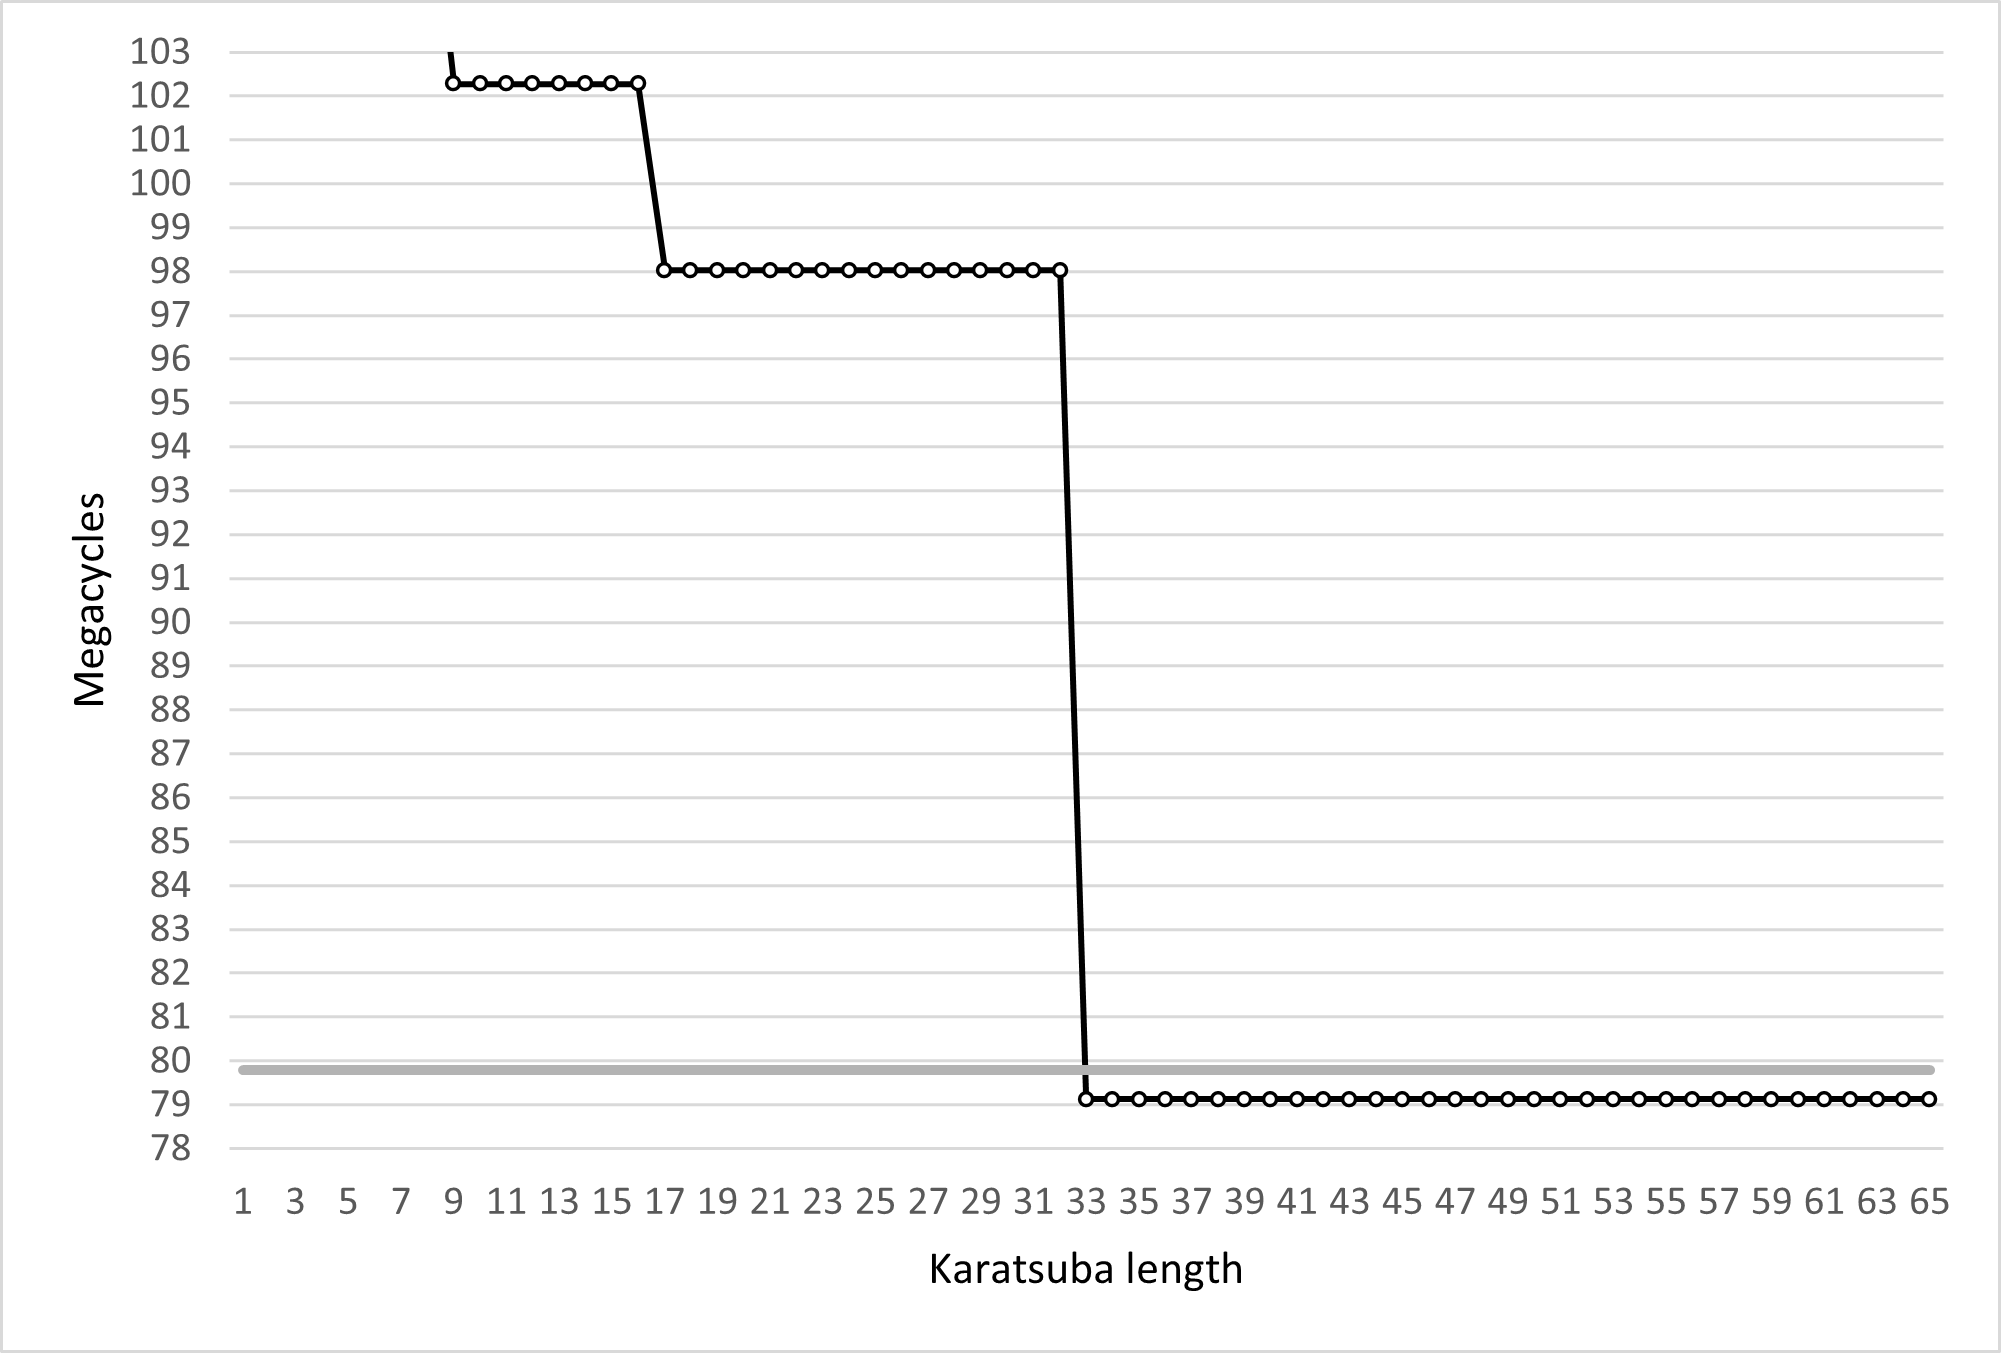
\includegraphics[width=0.8\textwidth]{report/images/karatsuba-compared.png}}
    \caption{Karatsuba operand lengths (black) compared to reference implementation (grey)}
\end{subfigure}
\label{karatsubacomparison}
\end{figure}

\subsection{Other tests}
%What other tests could have beeen usefull?